% 
% (c) Copyright 2016 Tabea Mendez
% 
% This source is free: you can redistribute it and/or modify
% it under the terms of the GNU General Public License as published by
% the Free Software Foundation, either version 3 of the License, or
% (at your option) any later version.
% 
% This source is distributed in the hope that it will be useful,
% but WITHOUT ANY WARRANTY; without even the implied warranty of
% MERCHANTABILITY or FITNESS FOR A PARTICULAR PURPOSE.  See the
% GNU General Public License for more details.
% 
% You should have received a copy of the GNU General Public License
% along with this source.  If not, see <http://www.gnu.org/licenses/>.
%
%%%%%%%%%%%%%%%%%%%%%%%%%%%%%%%%%%%%%%%%%%%%%%%%%%%%%%%%%%%%%%%%%%%%%%%%%%%%%%

Die Diskrete-Fourier-Transformation (DFT) und die Fast-Fourier-Transformation (FFT) ist für Folgendes von grosser Bedeutung:\\[-0.6cm]
\begin{itemize}
 \item Nummerische Berechnung des Frequenzspektrums eines Signals.\\[-0.6cm]
 \item Effiziente Berechnung der Faltung mittels FFT.\\[-0.6cm]
 \item Effiziente Speicherung und Übertragung von von Waveform-Signalen (Bilder und Sprache/Musik).
\end{itemize}

\section{Frequenzauflösung und Windowing}
	\begin{itemize}
	 \item Unendliches Signal $x(n)$ mittels eines Fensters auf eine endliche Länge reduzieren, um das Spektrum berechnen zu können.\\
		\begin{minipage}{0.5\textwidth}
			\fcolorbox{CadetRed}{white}{$x_L(n) = x(n)\cdot w(n)$}$\qquad$
			\fcolorbox{CadetRed}{white}{$T_L = L\cdot T = \dfrac{L}{f_s}$}
		\end{minipage}
		\begin{minipage}{0.3\textwidth}
			$\begin{array}{lcl}
			w(n): && \text{Fenster}\\
			x(n):&& \text{unendliches Signal}\\
			x_L(n):&& \text{endliches Signal}
			\end{array}$
		\end{minipage}
	 \item Die DTFT des windowed Signals kommt immer näher and die des orginalen unendlichen Signals, je länger das Fenster ist, bzw. je mehr Samples L verwendet werden.\\[0.2cm]
		\fcolorbox{CadetRed}{white}{$X(\omega) = \mysum{n=-\infty}{\infty}{x(n)\,\e^{-j\omega n}}\quad\approx\quad X_L(\omega) = \mysum{n=-\infty}{\infty}{x_L(n)\,\e^{-j\omega n}} = \mysum{n=0}{L-1}{x(n)\cdot w(n)\,\e^{-j\omega n}}$}\\
	 \item Durch das Windowing wird die \textbf{Frequenzauflösung reduziert}.\\[-0.5cm]
	 \item Das Windowing erzeugt \textbf{hohe Frequenzanteile im Spektrum} (frequency leakage)
	\end{itemize}
	
	\subsection{Rechteck-Fenster}
		\begin{tabularx}{\textwidth}{>{\centering\arraybackslash}p{7cm}c>{\centering\arraybackslash}X}
		 \textbf{Zeitbereich}&&\textbf{Frequenzbereich}\\[0.05cm]
		 \hline&&\\[-0.2cm]
		 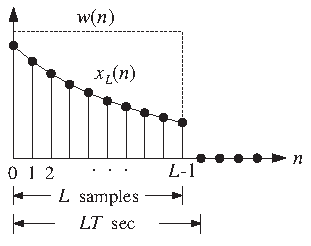
\includegraphics[height = 0.225\textwidth]{pic/rectangularWindowSamples.pdf}&&
		 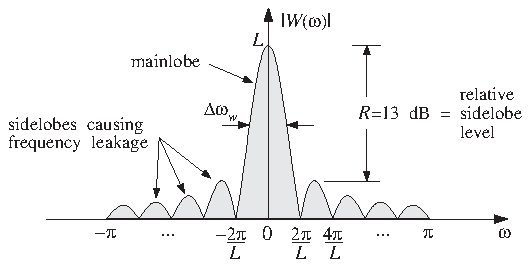
\includegraphics[height = 0.225\textwidth]{pic/rectangularWindow.pdf}\\
 		 \fcolorbox{CadetRed}{white}{$w(n) = \begin{cases}1,&0\leq n\leq L-1\\ 0,& \text{sonst}\end{cases}$} & \FT &
 		 \fcolorbox{CadetRed}{white}{$W(\omega) = \dfrac{1-\e^{-jL\omega}}{1-\e^{-j\omega}} = \dfrac{\sin(\omega L/2)}{\sin(\omega/2)}\cdot\e^{-j\omega (L-1)/2}$}\\[0.7cm]
		 \hline
		\end{tabularx} $ $\\

	\subsection{Hamming-Fenster}
		\begin{tabularx}{\textwidth}{p{0.5\textwidth}p{0.5\textwidth}}
		 \multicolumn{1}{c}{\textbf{Zeitbereich}}&\multicolumn{1}{c}{\textbf{Frequenzbereich}}\\[0.05cm]
		 \hline&\\[-0.6cm]
		 \multicolumn{1}{c}{\begin{minipage}{0.5\textwidth}
		 $\qquad\qquad$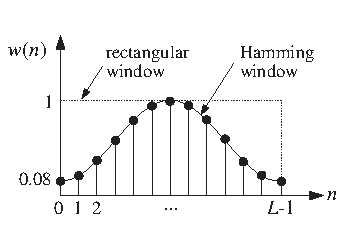
\includegraphics[width = 0.65\textwidth]{pic/hammingWindowSamples.pdf} \newline
		 \fcolorbox{CadetRed}{white}{$w(n) = \begin{cases}0.54-0.46\,\cos\left(\dfrac{2\pi n}{L-1}\right),&0\leq n\leq L-1\\ 0,& \text{sonst}\end{cases}$}
		 \end{minipage}}
		 &\multicolumn{1}{c}{\begin{minipage}{0.35\textwidth}
		 $ $\\$ $\\[0.2cm] 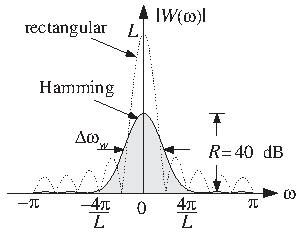
\includegraphics[width = \textwidth]{pic/hammingWindow.pdf}\end{minipage}}\\[2.9cm]
		 \hline
		\end{tabularx}
\newpage
	\subsection{Eigenschaften der Fenster-Spektren}\label{Eigenschaften der Fenster-Spektren}
		\begin{info}
		 Die Wahl des Fensters ist ein \textbf{Tradeoff} zwischen der Mainlobe-Width (Frequenzauflösung) und der Sidelobe-Suppression.
		\end{info}
		
		\begin{tabularx}{\textwidth}{|l|>{\centering\arraybackslash}X|>{\centering\arraybackslash}X|}
		 \hline&&\\[-0.3cm]
			& \textbf{Rechteck-Fenster} & \textbf{Hamming-Fenster}\\[0.1cm]
		 \hline&\multicolumn{2}{c|}{}\\[-0.3cm]
% 			Nullstellen & $\dfrac{2\pi k}{L}\quad k\neq 0$ & \\
			\textbf{Mainlobe} & \multicolumn{2}{c|}{Je grösser die Anzahl Samples $L$, desto höher und schmaler wird die Mainlobe.}\\&  \multicolumn{2}{c|}{(Die Sidelobes wachsen proportional mit.)}\\[0.1cm]
		\hline&\multicolumn{2}{c|}{}\\[-0.3cm]
			\textbf{Mainlobe-Width} &\multicolumn{2}{c|}{\fcolorbox{CadetRed}{white}{$\Delta\omega_W = c\cdot\dfrac{2\pi}{L} = c\cdot\dfrac{2\pi\Delta f_W}{f_s}$}}\\[0.6cm]
			&\multicolumn{2}{c|}{\fcolorbox{CadetRed}{white}{$\Delta f_W = c\cdot\dfrac{f_s}{L} = c\cdot\dfrac{1}{LT}= c\cdot\dfrac{1}{T_L}$} }\\[0.6cm]
			&\multicolumn{2}{c|}{$c\geq1$ }\\[0.15cm]
			& $c = 1\Rightarrow $ \textbf{Beste Frequenzauflösung} & $c = 2$\\[0.1cm]
		 \hline&&\\[-0.3cm]
			\textbf{Sidelobes} & Sind sehr gross, weil das Fenster im Zeitbereich scharf abschneidet.& Sind eher klein, weil das Fenster im Zeitbereich langsam hinein und hinaus fährt.\\[0.1cm]
		\hline&&\\[-0.3cm]
			\textbf{Sidelobe-Suppression} &\fcolorbox{CadetRed}{white}{$R = \left|\dfrac{W(\omega)}{W(0)}\right|_{\omega = 3\pi/L} \!\!\!\simeq \dfrac{2}{3\pi} \mathrel{\hat=} -13.46\db$}   & $\begin{array}{c}\text{\fcolorbox{CadetRed}{white}{$R =  -40\db$}}\\[0.2cm]\text{\textbf{$\Rightarrow$ gute Sidelobe-Suppression}}\end{array}$  \\[0.65cm]
		\hline
		\end{tabularx}$ $\\[0.2cm]

	\subsection{Frequenzauflösung}
		 Die Multiplikation des Signals $x(n)$ mit dem Fenster $w(n)$ entspricht im Frequenzbereich einer Faltung, wodurch das \textbf{Spektrum des Signals $X(\omega)$ verschmiert wird}.\\[0.2cm]
		 \fcolorbox{CadetRed}{white}{$x_L(n) = x(n) \cdot w(n)\qquad\FT\qquad X_L(\omega) = X(\omega) \ast W(\omega) = \frac{1}{2\pi}\myint{-\pi}{\pi}{X(\omega')\cdot W(\omega-\omega')}{\omega'}$}\\[0.5cm]
		 \textbf{Beispiel:}\\
		 $\begin{array}{rcl c rcl}
		 x(n) &= &A_1\,\e^{j\omega_1n} + A_2\,\e^{j\omega_2n}&\quad\FT&\quad
		 X(\omega) &= &\underline{\underline{2\pi\,A_1\,\delta(\omega-\omega_1) + 2\pi\,A_2\,\delta(\omega-\omega_2)}}\\[0.4cm]
		 x_L(n) & = & A_1\,\e^{j\omega_1n}\cdot w(n) + A_2\,\e^{j\omega_2n}\cdot w(n)&
		 \quad\FT &\quad X_L(\omega)&= &\;\;\;\;\!\myint{-\pi}{\pi}{A_1\,\delta(\omega'-\omega_1)\cdot W(\omega-\omega')}{\omega'} \\ &&&&&& + \myint{-\pi}{\pi}{A_2\,\delta(\omega'-\omega_2)\cdot W(\omega-\omega')}{\omega'}\\
		 &&&&&= & \underline{\underline{A_1\,W(\omega-\omega_1) + A_2\,W(\omega-\omega_2)}}
		 \end{array}$\\
		 \begin{minipage}{0.55\textwidth}
			$\begin{array}{ll}
			\Rightarrow& \textbf{Die Mainlobe muss schmaler sein, als der kleinste}\\ &\textbf{noch auflösbare Frequenzunterschied (Auflösung).}\\[0.2cm]
			&\text{\fcolorbox{CadetRed}{white}{$\Delta\omega \geq \Delta\omega_W = c\cdot\dfrac{2\pi}{L} = c\cdot\dfrac{2\pi\Delta f_W}{f_s}$}}\\[0.6cm]
			&\text{\fcolorbox{CadetRed}{white}{$\Delta f\geq \Delta f_W = c\cdot\dfrac{f_s}{L} = c\cdot\dfrac{1}{LT}= c\cdot\dfrac{1}{T_L}$}}\\[0.6cm]
			&\text{\fcolorbox{CadetRed}{white}{$L \geq c\cdot\dfrac{f_s}{\Delta f} = c\cdot\dfrac{2\pi}{\Delta \omega}$}}\end{array}$
		 \end{minipage}\begin{minipage}{0.05\textwidth}$ $\end{minipage}
		 \begin{minipage}{0.4\textwidth}
			$ $\\[1.5cm]
			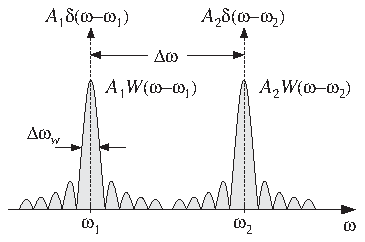
\includegraphics[width = 0.95\textwidth]{pic/frequenzaufloesung.pdf}
		 \end{minipage}
\newpage
\section{Discrete-Fourier-Transformation (DFT)}
	\begin{itemize}
	 \item Die Discrete-Time-Fourier-Transformation (DTFT) eines L-Sample langen Signals ist definiert als:\\[0.2cm]
	 \fcolorbox{CadetRed}{white}{$X(\omega) = \mysum{n=0}{L-1}{x(n)\,\e^{-j\omega n}}$}\\
	 \item Die Discrete-Fourier-Transformation (DFT) ist die DTFT, welche nur an bestimmten (diskreten) Frequenzpunkten ausgewertet wird. \\[-0.3cm]
	\end{itemize}
	
	\subsection{DFT für einzelne Frequenzen}
		\begin{itemize}
		\item Berechnung der DFT für einzelne bestimmte Frequenzen $\omega_i$ mittels der Übertragungsfunktion $H(z)$\\[0.2cm]
		\fcolorbox{CadetRed}{white}{$X(\omega_i) = \mysum{n=0}{L-1}{x(n)\,\e^{-j\omega_i n}} = \mysum{n=0}{L-1}{x(n)\,z^{-n}}|_{z = \e^{j\omega_i}} = X(z)|_{z = \e^{j\omega_i}}$}\\[0.2cm]
		$X(z) = x_0 + z^{-1}\cdot(x_1 + z^{-1}\cdot(x_2+z^{-1}\,x_3))$\\[-0.3cm]
		\end{itemize}
		
	\subsection{DFT für N-Frequenzen}
		\begin{itemize}
		 \item N-Point DFT eines L-Sample langen Signals mit N gleichmässig verteilten Frequenzpunkten.\\[0.2cm]
		\fcolorbox{CadetRed}{white}{$X(\omega_k) = \mysum{n=0}{L-1}{x(n)\,\e^{-j\omega_k n}} $}$\qquad$ mit $\quad \omega_k = \dfrac{2\pi k}{N}\qquad$ oder $\quad f_k = \dfrac{k\,f_s}{N}\qquad k = 0,1,...,N-1$\\[-0.3cm]
		\end{itemize}
		\begin{minipage}{0.7\textwidth}
		\begin{itemize}
		 \item Die N-Werte $X(\omega_k)$ können auch als Werte der z-Transformation\\ $X(z)$ auf dem Einheitskreis betrachtet werden\\[0.2cm]
		 \fcolorbox{CadetRed}{white}{$X(\omega_k) = X(z_k) = \mysum{n=0}{L-1}{x(n)\,z_k^{-n}} $}\\[0.4cm]
		 $z_k = \e^{j\omega_k} = \e^{2\pi jk/N}\qquad\quad k = 0,1,...,N-1$
		\end{itemize}
		\end{minipage}
		\begin{minipage}{0.4\textwidth} 
			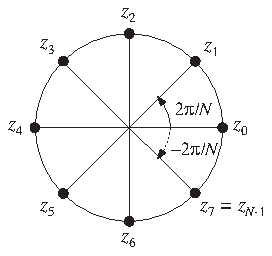
\includegraphics[width = 0.6\textwidth]{pic/dtftPeriodenKreis.pdf}
		\end{minipage}\\[-0.5cm]
		\begin{itemize}
		 \item Sie sind auch die N-ten Einheitswurzeln$\qquad$ \fcolorbox{CadetRed}{white}{$z^n = 1$}
		\end{itemize}$ $\\[-0.9cm]
		
	\subsection{Anzahl Frequenzpunkte versus Anzahl Samples}
		\begin{itemize}
		 \item \bm{$L$}: Anzahl Samples des Zeit-Signals $x(n)$
		 \item \bm{$N$}: Anzahl Samples des Frequenzspektrums $X(\omega)$
		 \item \bm{$L = N$}: Häufiger Spezialfall $\quad\Rightarrow\quad$ alles okej
		 \item \bm{$L < N$}: Zeitsequenz ist zu kurz $\quad\Rightarrow\quad$ am Ende des Signals Nullen anhängen (zero padding)
		 \item \bm{$L > N$}: Zeitsequenz ist zu lang $\quad\Rightarrow\quad$ überzählige Samples am Anfang addieren (modulo-N-wrapping\\ \hspace*{14cm}siehe Kapitel \ref{modNred})\\[-0.8cm]
		 \end{itemize}

	\subsection{Physikalische versus rechnerische Auflösung}
		\begin{minipage}{0.6\textwidth}
			\begin{tabularx}{\textwidth}{|>{\centering\arraybackslash}X|>{\centering\arraybackslash}X|}
			 \hline&\\[-0.3cm]
			 \textbf{Physikalische Auflösung} & \textbf{Rechnerische Auflösung}\\[0.1cm]
			 \hline&\\[-0.3cm]
				Frequenz-Differenz zwischen zwei noch unterscheidbaren Schwingungen aufgrund der Mainlobe-Width. & Frequenz-Differenz zwischen zwei Samples des abgetasteten Spektrums\\[0.1cm]
			 \hline&\\[-0.3cm]
				Beeinflussbar durch Anzahl Samples L des Zeit-Signals & Beeinflussbar durch Anzahl Samples N des Spektrums\\[0.1cm]
 			 \hline&\\[-0.3cm]
				\fcolorbox{CadetRed}{white}{$\Delta\omega_W = \dfrac{2\pi}{L}$}$\quad$\fcolorbox{CadetRed}{white}{$\Delta f_W = \dfrac{f_s}{L}$} & \fcolorbox{CadetRed}{white}{$\Delta\omega_{\text{bin}} = \dfrac{2\pi}{N}$}$\quad$\fcolorbox{CadetRed}{white}{$\Delta f_{\text{bin}} = \dfrac{f_s}{N}$}\\[0.5cm]
 			 \hline
			\end{tabularx}
		\end{minipage}\begin{minipage}{0.02\textwidth}$ $\end{minipage}
		\begin{minipage}{0.4\textwidth}
			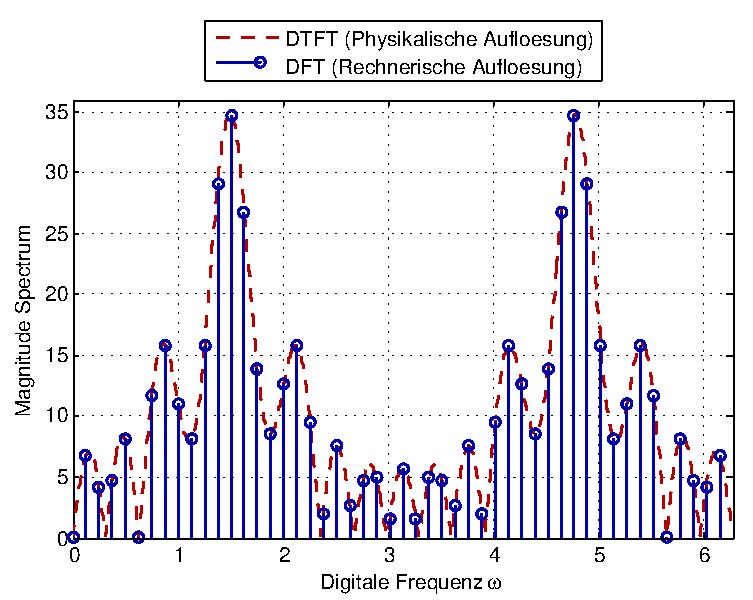
\includegraphics[width = \textwidth]{pic/phyVsComRes.pdf}
		\end{minipage}
\newpage
		\textbf{Mögliche Probleme des Frequenzspektrums}\\[0.2cm]
		\begin{minipage}{0.8\textwidth}
		\begin{itemize}
		 \item Die Samples der DFT fallen nicht zwangsweise auf die Peaks der DTFT. Denn die Samples stimmen nur dann exakt, wenn $k$ (DFT Index) eine ganze Zahl ist.\\
		 $\Rightarrow$ Rechnerische Auflösung erhöhen (Anzahl Samples $N$).
		\end{itemize}
		\end{minipage}\begin{minipage}{0.05\textwidth} $ $\end{minipage}
		\begin{minipage}{0.15\textwidth}
			\fcolorbox{CadetRed}{white}{$k = N\dfrac{f}{f_s}$}
		\end{minipage}
		\begin{itemize}
		 \item Der Frequenz Bias Fehler entsteht, wenn eine Mainlobe von fremden Sidelobes gestört wird (Interferenz) und sich dadurch der Peak der Mainlobe leicht verschiebt.\\
		 $\Rightarrow$ Physikalische Auflösung erhöhen (Anzahl Samples $L$).
		\end{itemize}

	\subsection{DFT als Matrix-Multiplikation}
		\begin{itemize}
		 \item Die Diskrete-Fourier-Transformation kann auch als Matrix-Multiplikation geschrieben werden:\\[0.2cm]
		\begin{minipage}{0.3\textwidth}
			\fcolorbox{CadetRed}{white}{$\bm{X} = \text{DFT}(\bm{x}) = \bm{A\cdot x} $}
		\end{minipage}
		\begin{minipage}{0.7\textwidth}
			Matrixelement: $\;\qquad A_{kn} = \e^{-j\omega_kn} = \e^{-j2\pi kn/N} = W_N^{kn}$\\
			Twiddle-Faktor: $\qquad W_N = \e^{-j2\pi/N}$ 
		\end{minipage}$ $\\[0.3cm]
		mit $\qquad\bm{X} = \begin{bmatrix}X(\omega_0)\\X(\omega_1)\\\vdots \\ X(\omega_{N-1})\end{bmatrix} = \begin{bmatrix}X_0\\X_1\\\vdots \\ X_{N-1}\end{bmatrix}\qquad$und$\qquad\bm{x} = \begin{bmatrix}x(0)\\x(1)\\\vdots \\ x(L-1)\end{bmatrix} = \begin{bmatrix}x_0\\x_1\\\vdots \\ x_{L-1}\end{bmatrix}$\\[0.3cm]
		und$\qquad\bm{A}
% 		= \begin{bmatrix} A_{00} & A_{01} & \dots & A_{0(L-1)}\\A_{10} & A_{11} & \dots & A_{1(L-1)}\\ \vdots& \vdots& \ddots& \vdots\\A_{(N-1)0} &A_{(N-1)1} & \dots & A_{(N-1)(L-1)}\end{bmatrix}
		= \begin{bmatrix} W_N^{0\cdot0} & W_N^{0\cdot1} & \dots & W_N^{0\cdot(L-1)}\\W_N^{1\cdot0} & W_N^{1\cdot1} & \dots & W_N^{1\cdot(L-1)}\\ \vdots& \vdots& \ddots& \vdots\\W_N^{(N-1)\cdot0} & W_N^{(N-1)\cdot1} & \dots & W_N^{(N-1)\cdot(L-1)}\end{bmatrix}
		= \begin{bmatrix} 1 & 1 & \dots & 1\\1 & W_N & \dots & W_N^{(L-1)}\\ \vdots& \vdots& \ddots& \vdots\\1 & W_N^{(N-1)} & \dots & W_N^{(N-1)(L-1)}\end{bmatrix}$\\[0.2cm]
		\end{itemize}
		\begin{minipage}{0.65\textwidth}
		\begin{itemize}
			\item Die Ermittlung der Matrix $\bm{A}$ bzw. der Twiddle-Faktoren $W_N^{kn}$ geht am einfachsten über den Einheitskreis der $z$-Ebene.\\[0.2cm]
			\fcolorbox{CadetRed}{white}{$W_N^k = \e^{-j2\pi k/N} = z_{-k}$}\\[-0.1cm]
			\begin{enumerate}
			 \item Matrix Zeilenweise auffüllen
			 \item Rechts bei $1$ beginnen und im Uhrzeigersinn die Werte des Einheitskreises eintragen.
			 \item Für die nächste Zeile wiederum rechts bei $1$ beginnen und im Uhrzeigersinn die Werte des Einheitskreises eintragen jedoch die Sprunglänge um eins erhöhen.
			 \item Schritt $3.$ so oft wiederholen bis die Matrix voll ist.
			\end{enumerate}
		\end{itemize}
		\end{minipage}\begin{minipage}{0.05\textwidth} $ $ \end{minipage}
		\begin{minipage}{0.3\textwidth}
			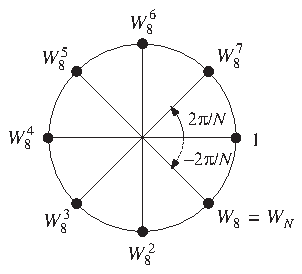
\includegraphics[width = \textwidth]{pic/twiddleFaktor.pdf}
		\end{minipage}$ $\\

		\begin{itemize}
		 \item Beispiel für eine DFT mit $N,L = 2$ und $4$\\
		 $\begin{bmatrix}X_0\\X_1\end{bmatrix} = \begin{bmatrix}1 & 1\\ 1 & -1 \end{bmatrix}\,\begin{bmatrix}x_0\\x_1\end{bmatrix} = \begin{bmatrix}x_0+x_1\\x_0-x_1\end{bmatrix}\qquad\qquad\qquad
		 \begin{bmatrix}X_0\\X_1\\X_2\\X_3\end{bmatrix} = \begin{bmatrix}1 & 1 & 1 & 1\\ 1 & -j &  -1 & j \\ 1&-1&1&-1\\1 & j & -1 & -j\end{bmatrix}\,\begin{bmatrix}x_0\\x_1\\x_2\\x_3\end{bmatrix}$\\[-0.3cm]
		\end{itemize}

	\subsection{Modulo-N Reduktion}\label{modNred}
		\begin{itemize}
		 \item Eine Modulo-N Reduktion des Eingangssignals (Eingangsvektor $\bm{x}$) ist notwendig wenn:\\[0.2cm]
		 \fcolorbox{CadetRed}{white}{Anzahl Zeit-Samples $L\;>\;$Anzahl Frequenz-Samples $N$}
		 \item Beim wrapping-Prozess wird der Vektor $\bm{x}$ in $N-$dimensionale Subvektoren unterteilt, die dann zusammengezählt werden. Wenn $L$ kein ganzzahliges Vielfaches von $N$ ist, wird $\bm{x}$ mit Nullen aufgefüllt.\\[0.2cm]
		 \begin{minipage}{0.47\textwidth}
			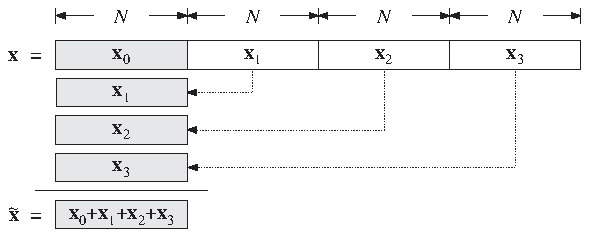
\includegraphics[width = \textwidth]{pic/modNred.pdf}
		 \end{minipage}
		 \begin{minipage}{0.53\textwidth}
			$\begin{array}{lcl}\widetilde x(n) & = & x_0(n) + x_1(n) + \hdots + x_{L/N-1}(n)\\[0.2cm] &=& x(n) + x(N+n) + \hdots + x((\frac{L}{N}-1)\cdot N + n)\end{array}$\\[0.2cm]
			$\Rightarrow\quad$\fcolorbox{CadetRed}{white}{$\widetilde x(n) = \mysum{m=0}{L/N-1}{x(m\,N+n)}$}$\quad n = 0,1,...,N-1$\\[0.2cm]
			$\Rightarrow\quad$\fcolorbox{CadetRed}{white}{$\widetilde{\bm{x}} = \bm{x}_0 + \bm{x}_1 + \hdots + \bm{x}_{(L/N)-1}$}
		 \end{minipage}
\newpage
		 \item Die N-Point-DFT des originalen, $L$-langen Signals $x(n)$ und die N-Point-DFT des modulo-$N$-gewrappten Signals $\widetilde x(n)$ sind identisch.\\[-0.4cm]
		 \begin{minipage}{0.35\textwidth}
		 \fcolorbox{CadetRed}{white}{$X(\omega_k) = \widetilde X(\omega_k)\quad\Rightarrow\quad X_k = \widetilde X_k$}\\[0.2cm]
			Also gilt auch:\\[0.2cm]
			\fcolorbox{CadetRed}{white}{$\begin{array}{lcl}\bm{X}& =& \bm{A}\,\bm{x} = \begin{bmatrix}\widetilde{\bm{A}} & \widetilde{\bm{A}} & \cdots\;\;\end{bmatrix}\,\begin{bmatrix}\bm{x}_0\\\bm{x}_1\\\vdots\end{bmatrix}\\[0.8cm]& = &  \widetilde{\bm{A}}\,(\bm{x}_0+\bm{x}_1+\hdots)\; = \;\widetilde{\bm{A}}\, \widetilde{\bm{x}} \; = \;\widetilde{\bm{X}}\end{array}$}
		 \end{minipage}
		 \begin{minipage}{0.6\textwidth}
			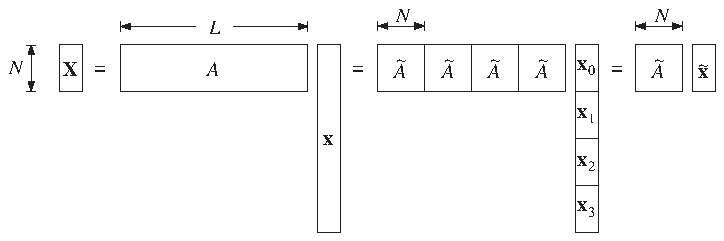
\includegraphics[width = \textwidth]{pic/modNredBeweis.pdf}\\[1.35cm]
		 \end{minipage}$ $\\[-0.4cm]
		 Dies ist bewiesen, wenn gezeigt werden kann, dass:$\quad$\fcolorbox{CadetRed}{white}{$\bm{A} = \begin{bmatrix}\bm{\widetilde A}&\bm{\widetilde A}&\bm{\widetilde A}&\cdots\;\;\end{bmatrix}\quad$ bzw. $\quad A_{kn} = A_{k(mN+n)}$}\\[0.2cm]
		 $\underline{\underline{A_{k(mN+n)}}} = W_N^{k(mN+n)} = W_N^{kmN}\cdot W_N^{kn} = (\e^{-j2\pi/N})^{kmN}\cdot W_N^{kn} = \underbrace{\e^{-j2\pi km}}_{1}\cdot W_N^{kn} = W_N^{kn} = \underline{\underline{A_{kn}}} $
		 \item Verschiedene Signale der Länge $L$ mit der selben modulo-$N$-Reduktion haben die gleiche $N$-Point-DFT.\\[0.2cm]
		 $\bm{x}\neq \bm{y}\;\cap \;\widetilde{\bm{x}} = \widetilde{\bm{y}}\quad\Rightarrow\quad X_k = Y_k$\\[0.2cm]
		 Diese Signale haben in der z-Domäne folgende Beziehung.\\[0.2cm]
		 $F(z_k) = X(z_k) - Y(z_k) = X_k - Y_k = 0\qquad k=0,1,...,N-1$\\[0.2cm]
		 Die $N$-Nullstellen auf dem Einheitskreis sind auch Nullstellen des Differenzpolynoms $F(z)$, womit gilt:\\[0.1cm]
		 $1-z^{-N} = \myprod{k=0}{N-1}{(1-z_k\,z^{-1})}\quad\Rightarrow\quad F(z) = X(z)-Y(z) = (1-z^{-N})\,Q(z)$\\[0.2cm]
		 $\Rightarrow\quad$\fcolorbox{CadetRed}{white}{$X(z) = Y(z) + (1-z^{-N})\,Q(z)$}$\qquad$ Ordnung von $Q(z)$ ist $(L-1)-N$\\[0.2cm]
		 $\Rightarrow\quad$\textbf{Zwei Sequenzen $x(n)$ und $y(n)$, die folgende Gleichung erfüllen haben, die selbe}\\  
		 \textcolor{white}{$\Rightarrow\quad$}\textbf{N-Point-DFT!}\\[0.2cm]
		 $\Rightarrow\quad$\fcolorbox{CadetRed}{white}{$x(n) = y(n) + q(n) - q(n-N)$}$\qquad n=0,1,...,L-1$
		\end{itemize}$ $\\[-1cm]

	\subsection{Inverse-Discrete-Fourier-Transformation (IDFT)}
		$ $\\[-1.2cm]
		\begin{minipage}{0.6\textwidth}
		\begin{itemize}
			\item $\begin{array}{l}\!\!\!\text{Die Discrete-Fourier-Transformation kann geschrieben werden als:}\end{array}$\\
			$\bm{X} = \bm{A\,x} = \bm{\widetilde A\,\widetilde x}$\\[-0.3cm]
			\item $\begin{array}{l}\!\!\!\text{Damit ist die Inverse-Discrete-Fourier-Transformation folgendes:}\end{array}$\\[0.2cm]
			\fcolorbox{CadetRed}{white}{$\widetilde{\bm{x}} = \text{IDFT}(\bm{X}) = \bm{\widetilde A^{-1}\, X}$}\\[0.3cm]
			\begin{danger}
			Damit die Matrix $\bm{A}$ invertierbar ist, muss sie symetrisch sein, was bei der Matrix $\widetilde{\bm{A}}$ gegeben ist. Somit kann die IDFT nur das modulo-$N$-gewrappte Signal $\widetilde{x}$ bzw. $\widetilde{x}(n)$ rekonstruieren!
			\end{danger}\\[0.1cm]
			Dabei gilt jedoch:$\qquad$
			\fcolorbox{CadetRed}{white}{$\begin{array}{lcl}\widetilde{\bm{x}} = \bm{x}&&\text{wenn }N\geq L\\\widetilde{\bm{x}} \neq \bm{x}&&\text{wenn }N<L\\&&\Rightarrow\;\text{ Aliasing im Frequenzbereich!}\end{array}$}
		\end{itemize}
		\end{minipage}\begin{minipage}{0.05\textwidth} $ $\end{minipage}
		\begin{minipage}{0.35\textwidth}
			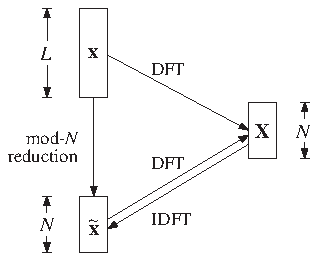
\includegraphics[width = \textwidth]{pic/idft.pdf}\\[3cm]	
		\end{minipage}$ $\\[-0.5cm]
		\begin{tabular}{cll}
			 $\quad\bullet\!\!\!\!$& Aufgrund der Beziehung & \fcolorbox{CadetRed}{white}{$\dfrac{1}{N}\,\widetilde{\bm{A}}\,\widetilde{\bm{A}}^\ast = \bm{I}_N\qquad\Rightarrow\qquad \widetilde{\bm{A}}^{-1} = \dfrac{1}{N}\,\widetilde{\bm{A}}^\ast$}\\[0.45cm]
			&kann die IDFT vereinfacht werden zu & \fcolorbox{CadetRed}{white}{$\widetilde{\bm{x}} = \text{IDFT}(\bm{X}) =\dfrac{1}{N}\,\widetilde{\bm{A}}^\ast \, \bm{X}$}\\[0.45cm]
			&oder mit der DFT geschrieben werden als $\qquad$& \fcolorbox{CadetRed}{white}{$\widetilde{\bm{x}} = \text{IDFT}(\bm{X}) =\dfrac{1}{N}\,\big[\text{DFT}(\bm{X}^{\ast})\big]^\ast$}\\		
		\end{tabular}
\newpage
	\subsection{DTFT/IDTFT versus DFT/IDFT}
		\begin{tabularx}{\textwidth}{|p{4.2cm}|X|X|}
		\hline&&\\[-0.25cm]
			&\textbf{DTFT/IDTFT} & \textbf{DFT/IDFT}\\[0.1cm]
		\hline&&\\[-0.25cm]
			Fourier-Transformation: &
			$\bullet\;$ $L$ Zeit-Samples\newline 
			$\bullet\;$ $\infty$ Frequenz-Samples\newline 
			$\bullet\;$ $\begin{array}{l}\\[-0.3cm]\!\!\!\text{\fcolorbox{CadetRed}{white}{$X(\omega) = \mysum{n=0}{L-1}{x(n)\,\e^{-j\omega n}}$}}\end{array}$&
			$\bullet\;$ $L$ Zeit-Samples\newline 
			$\bullet\;$ $N$ Frequenz-Samples\newline 
			$\bullet\;$ $\begin{array}{l}\\[-0.3cm]\!\!\!\text{\fcolorbox{CadetRed}{white}{$X(\omega_k) = \mysum{n=0}{L-1}{x(n)\,\e^{-j\omega_k n}}$}}\end{array}$\\[0.7cm]
		\hline&&\\[-0.25cm]
			Inverse-Fourier-Transformation: &
			$\bullet\;$ Rekonstruiert das gesamte\newline \textcolor{white}{$\bullet\;$} originale Signal $x(n)$\newline 
			$\bullet\;$ $\begin{array}{l}\\[-0.3cm]\!\!\!\text{\fcolorbox{CadetRed}{white}{$x(n) = \dfrac{1}{2\pi}\myint{0}{2\pi}{X(\omega)\,\e^{j\omega n}}{\omega}$}}\end{array}$&
			$\bullet\;$ Rekonstruiert nur das\newline \textcolor{white}{$\bullet\;$} modulo-$N$-gewrappte Signal $\widetilde{x}(n)$\newline 
			$\bullet\;$ $\begin{array}{l}\\[-0.3cm]\!\!\!\text{\fcolorbox{CadetRed}{white}{$\widetilde x(n) = \dfrac{1}{N}\mysum{k=0}{N-1}{X(\omega_k)\,\e^{j\omega_k n}}$}}\end{array}$\\[0.7cm]
		\hline&\multicolumn{2}{X|}{ }\\[-0.25cm]
			$\begin{array}{l}\!\!\!\text{IDFT als Approximation}\\\!\!\!\text{der IDTFT:}\end{array}$& 
			\multicolumn{2}{l|}{$x(n)\; = \;\dfrac{1}{2\pi}\myint{0}{2\pi}{X(\omega)\,\e^{j\omega n}}{\omega}\;\simeq\; \mysum{k=0}{N-1}{X(\omega_k)\,\e^{j\omega_k n}}\,\dfrac{\Delta\omega_{\text{bin}}}{2\pi} \; = \; \dfrac{1}{N}\mysum{k=0}{N-1}{X(\omega_k)\,\e^{j\omega_k n}}$}\\[0.4cm]
		\hline
		\end{tabularx}
	
\section{Fast-Fourier-Transformation (FFT)}
	\begin{itemize}
	 \item Die Fast-Fourier-Transformation (FFT) ist eine schnelle Implementation der Discrete-Fourier-Trans-formation (DFT), welche $N^2$ komplexe Multiplikation benötigen würde. \textbf{Somit sind die Resultate der FFT und der DFT identisch.}
	 \item Die FFT berechnet die DFT mit der ''Teile-und-Hersche'' Strategie, daher ist es von Vorteil, wenn die Anzahl Frequenz-Samples eine Zweierpotenz ist.\\[0.2cm]
	 \fcolorbox{CadetRed}{white}{$N = 2^B\qquad\Rightarrow\qquad B = \log_2(N)$}\\[-0.25cm]
	 \item Bei der FFT muss die Anzahl Zeit-Samples $L$ und die Anzahl Frequenz-Samples $N$ gleich gross sein. Ist dies nicht der Fall, so muss das Zeitsignal vorverarbeitet werden (Zero-Padding oder modulo-N-wrapping).\\[0.2cm]
	 \fcolorbox{CadetRed}{white}{$N = L$}\\[-0.2cm]
	\end{itemize}
	
	\subsection{Teile-und-Hersche Strategie}
		\begin{minipage}{0.7\textwidth}
		\begin{itemize}
		 \item Das Problem der Berechnung einer $N$-Point-DFT wird reduziert auf die Berechnung von zwei $N/2$-Point-DFTs.\\[0.2cm]
		 \fcolorbox{CadetRed}{white}{$N$ - Point - DFT$\;=\; 2\cdot \dfrac{N}{2}$ - Point - DFT$\;+\; \dfrac{N}{2}$ komplexe Multiplikationen}\\[0.2cm]
		 \item Die $N/2$-Point-DFTs wiederum in $N/4$-Point-DFTs aufteilen, usw.\\[-0.2cm]
		 \item Wenn die $N$-Point-DFT über $m$ Stufen aus $N/2^m$-Point-DFTs berechnet wird, sind $M$ komplexe Multiplikation notwendig.\\[0.2cm]
		 \fcolorbox{CadetRed}{white}{$ M\;  =\; \dfrac{N^2}{2^m} + \dfrac{N}{2}m\; =\; \underbrace{2^m\left(\dfrac{N}{2^m}\right)^2 }_{\text{DFT}} + \underbrace{2^{m-1}\dfrac{N}{2^m} +\hdots  + 4\dfrac{N}{8} + 2\dfrac{N}{4} + \dfrac{N}{2}}_{\text{Stufen-Multiplikationen}}$}\\[0.25cm]
		 \item Wenn mit $1$-Point-DFTs gestartet wird sind $m = B = \log_2(N)$ Stufen notwendig und die Berechnung der $1$-Point-DFTs entfällt, weil diese gerade sich selbst entsprechen. Damit entfällt der erste Term und es müssen nur noch die Stufen-Multiplikationen berechnet werden.\\[0.2cm]
		 \fcolorbox{CadetRed}{white}{$ M\; =\; \dfrac{N}{2}m\; =\; \dfrac{1}{2}NB\; = \;\dfrac{1}{2}N\log_2(N)$}
		\end{itemize}
		\end{minipage}\begin{minipage}{0.05\textwidth}$ $\end{minipage}
		\begin{minipage}{0.25\textwidth}
			\hspace*{0.25cm}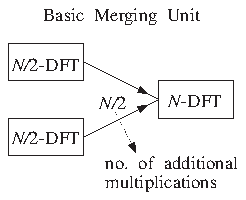
\includegraphics[width = 0.9\textwidth]{pic/multistageDFTeinheit.pdf}\\
			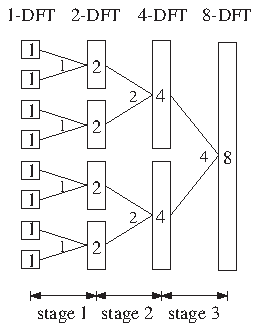
\includegraphics[width = \textwidth]{pic/multistageDFT.pdf}
		\end{minipage}
\newpage
	\subsection{$\bm{N}$-Point-DFT aus zwei $\bm{N/2}$-Point-DFTs berechnen}
		\begin{itemize}
		 \item Aufsplittung der DFT $X(k)$ in zwei Terme $G(k)$ und $H(k)$ welche jeweils die geraden bzw. die ungeraden Samples der Zeit-Sequenz berücksichtigen.\\[0.2cm]
		 $\begin{array}{lclcl}
		 X(k)& =& \mysum{n=0}{N-1}{x(n)\,\e^{-j\omega_k n}}\;\; =\;\; \mysum{n=0}{N-1}{W_N^{k n}\,x(n)} &&\\[0.5cm]
		 & =& \mysum{n=0}{N/2-1}{W_N^{k(2n)}\,x(2n)} + \mysum{n=0}{N/2-1}{W_N^{k(2n+1)}\,x(2n+1)}& &\Big|\;\;\text{\fcolorbox{CadetRed}{white}{$\begin{array}{lcl}g(n)\!\!\!\! & =\!\!\!\! & x(2n)\\h(n)\!\!\!\! & =\!\!\!\! & x(2n+1)\end{array}$}}\quad n = 0,1,...,\frac{N}{2}-1 \\[0.6cm]
		 & =&\mysum{n=0}{N/2-1}{W_N^{k(2n)}\,g(n)} + \mysum{n=0}{N/2-1}{W_N^{k(2n+1)}\,h(n)} & &\Big|\;\;W_N^{2} = W_{N/2} \\[0.6cm]
		 & =& \mysum{n=0}{N/2-1}{W_{N/2}^{kn}\,g(n)} + \mysum{n=0}{N/2-1}{W_N^{k}\,W_{N/2}^{kn}\,h(n)} & &\\[0.6cm]
		 & =&\underline{\underline{G(k) + W_N^{k}\,H(k)}} & & \\[0.6cm]
		 \end{array}$\\[-0.2cm]
		 $\begin{array}{ll}\Rightarrow&\quad\text{\fcolorbox{CadetRed}{white}{$X(k) = G(k) + W_N^{k}\,H(k)$}$\qquad$ mit}\\[0.2cm]&\quad N-\text{periodisch}\\[0.1cm]&\qquad\rightarrow\quad k=0,1,...,N-1\end{array}$
		 $\qquad $\fcolorbox{CadetRed}{white}{$\begin{array}{lcl}G(k)\!\!\!\! & =\!\!\!\! & \mysum{n=0}{N/2-1}{W_{N/2}^{kn}\,g(n)}\\[0.35cm] H(k)\!\!\!\! & =\!\!\!\! & \mysum{n=0}{N/2-1}{W_{N/2}^{kn}\,h(n)}\end{array}$}$\;\;$
		  $\begin{array}{l}N/2-\text{periodisch}\\[0.1cm]\quad\rightarrow\quad k = 0,1,...,\frac{N}{2}-1\end{array}$
		 \item Um die Anzahl Multiplikation mit $W_N^k$ noch zu halbieren, wird die Eigenschaft ausgenutzt, dass $G(k)$ und $H(k)$ mit $N/2$ periodisch sind.\\[0.2cm]
		 $\begin{array}{lclcl}
		 X(k)& =& \underline{G(k) + W_N^{k}\,H(k)} &&\Big|\;\; k = 0,1,...,\frac{N}{2}-1\\[0.2cm]
		 X(k+\frac{N}{2})& =& G(k+\frac{N}{2}) + W_N^{k+N/2}\,H(k+\frac{N}{2}) &&\Big|\;\; G(k+\frac{N}{2}) = G(k)\quad\text{und}\quad H(k+\frac{N}{2}) = H(k)\\[0.2cm] 
 		 & =& G(k) + W_N^{k}\,W_N^{N/2}\,H(k) &&\Big|\;\; W_N^{N/2} = -1\\[0.2cm]
 		 & =& \underline{G(k) - W_N^{k}\,H(k)} &&
 		 \end{array}$\\[0.5cm]
		 $\Rightarrow\qquad$\fcolorbox{CadetRed}{white}{
		 $\begin{array}{lcl}
		 X(k)& =& G(k) + W_N^{k}\,H(k)\\[0.2cm]
		 X(k+\frac{N}{2})& =& G(k) - W_N^{k}\,H(k)
		 \end{array}$}$\qquad k = 0,1,...,\frac{N}{2}-1$
		 \item Somit kann eine  $N$-Point-DFT folgendermassen aus zwei $N/2$-Point-DFTs berechnet werden.\\[0.2cm]
		 \begin{minipage}{0.6\textwidth}
			\fcolorbox{CadetRed}{white}{$X(k) = 
			\begin{cases}
			\begin{bmatrix}X_0 \\ X_1\\\vdots\\X_{N/2-1}\end{bmatrix} 
			= \begin{bmatrix}G_0 \\ G_1\\\vdots\\G_{N/2-1}\end{bmatrix}
			+ \begin{bmatrix}H_0 \\ H_1\\\vdots\\H_{N/2-1}\end{bmatrix}
			\times \begin{bmatrix}W_N^0 \\ W_N^1\\\vdots\\W_N^{N/2-1}\end{bmatrix} \\
			\begin{bmatrix}X_{N/2} \\ X_{N/2+1}\\\vdots\\X_{N-1}\end{bmatrix} 
			= \begin{bmatrix}G_0 \\ G_1\\\vdots\\G_{N/2-1}\end{bmatrix}
			+ \begin{bmatrix}H_0 \\ H_1\\\vdots\\H_{N/2-1}\end{bmatrix}
			\times \begin{bmatrix}W_N^0 \\ W_N^1\\\vdots\\W_N^{N/2-1}\end{bmatrix}
			\end{cases}$}
		 \end{minipage}
		 \begin{minipage}{0.35\textwidth}
			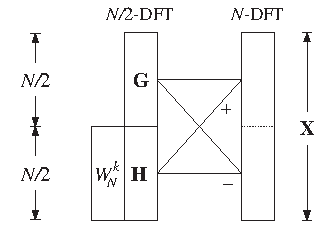
\includegraphics[width = \textwidth]{pic/N2toNdft.pdf}
		 \end{minipage}
		 
		\end{itemize}
\newpage
	\subsection{FFT-Algorithmus}
		\begin{itemize}
		 \item Der Eingang muss in gerade und ungerade Sequenzen unterteilt werden. Dies muss so oft wiederholt werden, bis nur noch ein Element übrig bleibt.\\[0.1cm]
		 \begin{minipage}{0.4\textwidth}
			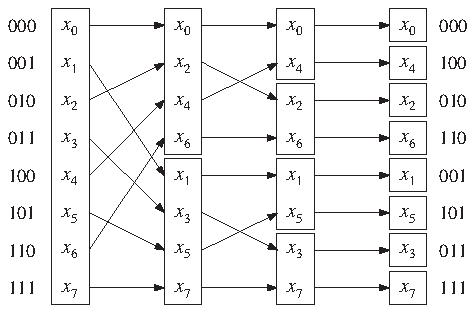
\includegraphics[width = \textwidth]{pic/andrdnungfuerFFT.pdf}
		 \end{minipage}
		 \begin{minipage}{0.55\textwidth}
			\begin{tabularx}{\textwidth}{llX}
				&$\Rightarrow\quad$ & Das richtige Anordnen der Werte für die FFT wird auch als \textbf{Bit-Reversal} bezeichnet, weil der binäre Startindex rückwärts gelesen gerade dem binären Zielindex entspricht.\\
				&&Bsp: $011\quad\rightarrow\quad 110$\\
			\end{tabularx}			
		 \end{minipage}
		 \item Wenn alle Eingangssamples richtig geordnet sind, kann der FFT-Algorithmus darauf angewendet werden.\\[0.1cm]
		 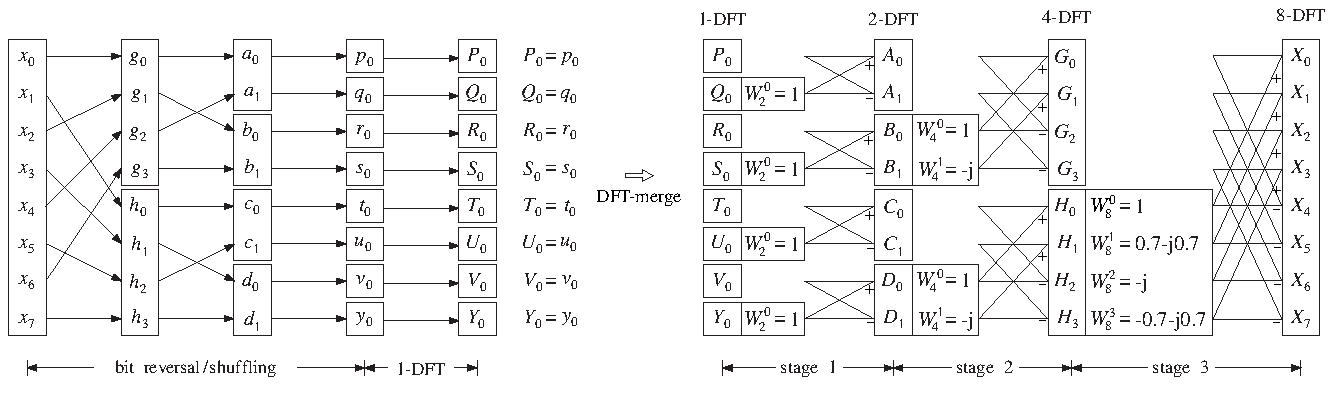
\includegraphics[width = 0.95\textwidth]{pic/FFTAlg.pdf}
		\end{itemize}

	
\section{Schnelle Faltung mit FFT}
	\begin{itemize}
	 \item Eine fundamentale Beziehung zwischen Zeit- und Frequenzbereich ist\\[0.2cm]
	 \fcolorbox{CadetRed}{white}{$\bm{y} = \bm{h}\ast\bm{ x}\qquad\Leftrightarrow\qquad Y(\omega) = H(\omega)\cdot X(\omega)$}\\[-0.3cm]
	 \item Um also die Faltung möglichst effizient berechnen zu können, kann die FFT/IFFT verwendet werden.\\[0.2cm]
	 \fcolorbox{CadetRed}{white}{$\widetilde{\bm{y}} = \widetilde{\bm{h\ast x}} =\text{IDFT}\big[\text{DFT}({\bm{h}})\cdot\text{DFT}({\bm{x}})\big]$}
	 \item Da mit der FFT/IFFT jedoch nur die \textbf{Zirkulare Faltung} (modulo-$N$-gewrappte Version) berechnet werden kann, müssen die beiden Eingangssignale $x(n)$ und $h(n)$ mit Nullen aufgefüllt werden.\\[0.2cm]
	 \begin{tabular}{|c|c|c|}
	  \hline&&\\[-0.3cm]
		Signal: & ursprüngliche Länge & Zero-Padded Länge\\[0.1cm]
	  \hline&&\\[-0.3cm]
		$\bm{x}$ & $L$ & $L_y =  L+M$\\
		$\bm{h}$ & $M+1$ (Ordnung $M$) & $L_y = L+M$\\[0.1cm]
	  \hline
	 \end{tabular}$\qquad\Rightarrow\qquad$\fcolorbox{CadetRed}{white}{$\widetilde{\bm{y}} = \bm{y}\;\;$ wenn $N\geq L_y = L+M$ }\\
	 \item Die rechnerischen Kosten dafür sind $\dfrac{3}{2}N\log_2(N) + N$ komplexe Multiplikationen
	\end{itemize}
	
	\subsection{Overlap-Add-Faltung}
			\begin{itemize}
			 \item Unendlich langes Signal $x(n)$ muss mit einem Filter $h(n)$ gefaltet werden.\\[-0.42cm]
			 \end{itemize}
		\begin{minipage}{0.55\textwidth}
			\begin{itemize}
			 \item Signal wird in $L$ lange Eingangsblöcke zerlegt, die einzeln mittels FFT und IFFT gefaltet werden.\\[-0.4cm]
			 \item Durch die Faltung entstehen $L+M$ lange Ausgangsblöcke, von welchen nur die ersten $L$ Samples direkt verwendet werden und die letzten $M$ Samples in einem Buffer $\bm{y}_\text{temp}$ zwischengespeichert werden.\\[-0.4cm]
			 \item Die Samples des Zwischenspeichers $\bm{y}_\text{temp}$ werden beim nächsten Ausgangsblock vorne addiert.
			\end{itemize}
		\end{minipage}\begin{minipage}{0.02\textwidth}$ $\end{minipage}
		\begin{minipage}{0.45\textwidth}
			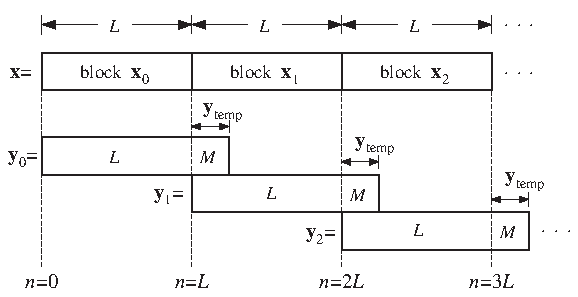
\includegraphics[width = \textwidth]{pic/overlapAdd.pdf}
		\end{minipage}
\newpage
	\subsection{Overlap-Save-Faltung}
		\begin{itemize}
			 \item Unendlich langes Signal $x(n)$ muss mit einem Filter $h(n)$ gefaltet werden.
			 \item Signal wird in $L$ lange Eingangsblöcke zerlegt, welche jeweils um $M$ Samples überlappen.
			 \item Die $L$ langen Eingangsblöcke werden ohne Zero-Padding mittels FFT und IFFT gefaltet, wodurch, aufgrund der Circularen Faltung, $L$ lange Ausgangsblöcke entstehen. Bei diesen Ausgangsblöcken sind jedoch die ersten $M$ Samples falsch.
			 \item Diese falschen Samples werden jedoch verworfen, da die richtigen Samples bereits vom vorhergehenden Ausgangsblock berechnet wurden.\\[0.3cm]
			 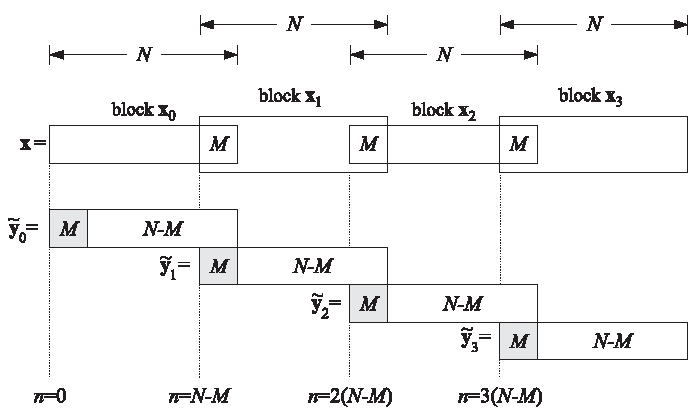
\includegraphics[width = 0.5\textwidth]{pic/overlapSave.pdf}
		\end{itemize}